%% fig_kahlersign.tex   (generated by make_round11.py; do not edit by hand)
%% The sign of int gamma kappa^2 on the Kaehler cone at n = 2.
\documentclass[tikz,border=8pt]{standalone}
\usepackage{amsmath,amssymb}
\usetikzlibrary{arrows.meta,calc,decorations.pathreplacing}
%% palette.tex -- shared colour definitions for the figures
\definecolor{PInk}{RGB}{26,32,44}
\definecolor{PBlue}{RGB}{37,82,139}
\definecolor{PTeal}{RGB}{23,127,125}
\definecolor{POchre}{RGB}{193,138,44}
\definecolor{PClay}{RGB}{178,74,58}
\definecolor{PSlate}{RGB}{108,122,137}
\definecolor{PViolet}{RGB}{110,86,150}
\definecolor{WBlue}{RGB}{223,234,246}
\definecolor{WTeal}{RGB}{220,238,236}
\definecolor{WOchre}{RGB}{250,240,218}
\definecolor{WClay}{RGB}{247,229,224}
\definecolor{WSlate}{RGB}{238,241,244}
\definecolor{PMag}{RGB}{158,58,110}
\definecolor{PGrass}{RGB}{62,124,66}
\definecolor{PAmber}{RGB}{214,112,38}
\definecolor{PIndigo}{RGB}{58,64,140}
\definecolor{PRule}{RGB}{176,186,197}

%% shared macros so the standalone figures match the paper
\providecommand{\QQ}{\mathbb{Q}}
\providecommand{\ZZ}{\mathbb{Z}}
\providecommand{\RR}{\mathbb{R}}
\providecommand{\CC}{\mathbb{C}}
\providecommand{\PP}{\mathbb{P}}
\providecommand{\Kx}{K^{\times}}
\providecommand{\HW}{W}
\providecommand{\Nm}{\mathrm{N}}
\providecommand{\Hdg}{\mathrm{Hdg}}
\providecommand{\NS}{\mathrm{NS}}
\providecommand{\cA}{\mathcal{A}}
\providecommand{\cD}{\mathcal{D}}
\providecommand{\cF}{\mathcal{F}}
\providecommand{\cP}{\mathcal{P}}
\providecommand{\cO}{\mathcal{O}}
\providecommand{\cQ}{\mathcal{Q}}
\providecommand{\bbar}[1]{\overline{#1}}
\providecommand{\ch}{\operatorname{ch}}
\providecommand{\End}{\mathrm{End}}

\begin{document}
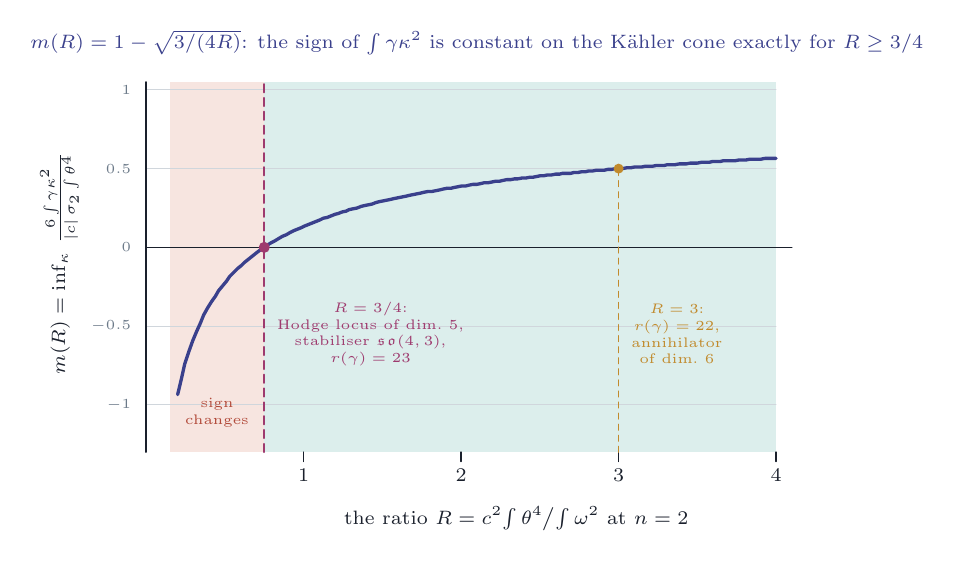
\begin{tikzpicture}[x=1cm,y=1cm,line join=round,line cap=round,
  font=\small,text=PInk]
  \fill[WClay] (0.30,-2.60) rectangle (1.50,2.10);
  \fill[WTeal] (1.50,-2.60) rectangle (8.00,2.10);
  \draw[PRule!60,line width=0.30pt] (0.00,-2.00) -- (8.00,-2.00);
  \node[text=PSlate,inner sep=1pt,align=center,font=\tiny,anchor=east] at (-0.15,-2.00) {$-1$};
  \draw[PRule!60,line width=0.30pt] (0.00,-1.00) -- (8.00,-1.00);
  \node[text=PSlate,inner sep=1pt,align=center,font=\tiny,anchor=east] at (-0.15,-1.00) {$-0.5$};
  \draw[PRule!60,line width=0.30pt] (0.00,1.00) -- (8.00,1.00);
  \node[text=PSlate,inner sep=1pt,align=center,font=\tiny,anchor=east] at (-0.15,1.00) {$0.5$};
  \draw[PRule!60,line width=0.30pt] (0.00,2.00) -- (8.00,2.00);
  \node[text=PSlate,inner sep=1pt,align=center,font=\tiny,anchor=east] at (-0.15,2.00) {$1$};
  \draw[PInk,line width=0.60pt] (0.00,0.00) -- (8.20,0.00);
  \node[text=PSlate,inner sep=1pt,align=center,font=\tiny,anchor=east] at (-0.15,0.00) {$0$};
  \draw[PInk,line width=0.60pt] (0.00,-2.60) -- (0.00,2.10);
  \draw[PInk,line width=0.50pt] (2.00,-2.60) -- (2.00,-2.72);
  \node[text=PInk,inner sep=1pt,align=center,font=\scriptsize] at (2.00,-2.90) {$1$};
  \draw[PInk,line width=0.50pt] (4.00,-2.60) -- (4.00,-2.72);
  \node[text=PInk,inner sep=1pt,align=center,font=\scriptsize] at (4.00,-2.90) {$2$};
  \draw[PInk,line width=0.50pt] (6.00,-2.60) -- (6.00,-2.72);
  \node[text=PInk,inner sep=1pt,align=center,font=\scriptsize] at (6.00,-2.90) {$3$};
  \draw[PInk,line width=0.50pt] (8.00,-2.60) -- (8.00,-2.72);
  \node[text=PInk,inner sep=1pt,align=center,font=\scriptsize] at (8.00,-2.90) {$4$};
  \draw[PIndigo,line width=1.20pt] (0.40,-1.87) -- (0.45,-1.66) -- (0.49,-1.48) -- (0.54,-1.33) -- (0.59,-1.19) -- (0.64,-1.07) -- (0.69,-0.96) -- (0.73,-0.86) -- (0.78,-0.77) -- (0.83,-0.69) -- (0.88,-0.62) -- (0.92,-0.55) -- (0.97,-0.49) -- (1.02,-0.43) -- (1.06,-0.37) -- (1.11,-0.32) -- (1.16,-0.27) -- (1.21,-0.23) -- (1.25,-0.19) -- (1.30,-0.15) -- (1.35,-0.11) -- (1.40,-0.07) -- (1.44,-0.04) -- (1.49,-0.01) -- (1.54,0.03) -- (1.59,0.06) -- (1.63,0.08) -- (1.68,0.11) -- (1.73,0.14) -- (1.78,0.16) -- (1.83,0.19) -- (1.87,0.21) -- (1.92,0.23) -- (1.97,0.25) -- (2.01,0.27) -- (2.06,0.29) -- (2.11,0.31) -- (2.16,0.33) -- (2.21,0.35) -- (2.25,0.37) -- (2.30,0.38) -- (2.35,0.40) -- (2.40,0.42) -- (2.44,0.43) -- (2.49,0.45) -- (2.54,0.46) -- (2.58,0.48) -- (2.63,0.49) -- (2.68,0.50) -- (2.73,0.52) -- (2.77,0.53) -- (2.82,0.54) -- (2.87,0.55) -- (2.92,0.57) -- (2.96,0.58) -- (3.01,0.59) -- (3.06,0.60) -- (3.11,0.61) -- (3.15,0.62) -- (3.20,0.63) -- (3.25,0.64) -- (3.30,0.65) -- (3.34,0.66) -- (3.39,0.67) -- (3.44,0.68) -- (3.49,0.69) -- (3.53,0.70) -- (3.58,0.71) -- (3.63,0.71) -- (3.68,0.72) -- (3.73,0.73) -- (3.77,0.74) -- (3.82,0.75) -- (3.87,0.75) -- (3.91,0.76) -- (3.96,0.77) -- (4.01,0.78) -- (4.06,0.78) -- (4.10,0.79) -- (4.15,0.80) -- (4.20,0.80) -- (4.25,0.81) -- (4.29,0.82) -- (4.34,0.82) -- (4.39,0.83) -- (4.44,0.84) -- (4.49,0.84) -- (4.53,0.85) -- (4.58,0.86) -- (4.63,0.86) -- (4.68,0.87) -- (4.72,0.87) -- (4.77,0.88) -- (4.82,0.88) -- (4.87,0.89) -- (4.91,0.89) -- (4.96,0.90) -- (5.01,0.91) -- (5.05,0.91) -- (5.10,0.92) -- (5.15,0.92) -- (5.20,0.93) -- (5.25,0.93) -- (5.29,0.94) -- (5.34,0.94) -- (5.39,0.94) -- (5.43,0.95) -- (5.48,0.95) -- (5.53,0.96) -- (5.58,0.96) -- (5.62,0.97) -- (5.67,0.97) -- (5.72,0.98) -- (5.77,0.98) -- (5.82,0.98) -- (5.86,0.99) -- (5.91,0.99) -- (5.96,1.00) -- (6.00,1.00) -- (6.05,1.00) -- (6.10,1.01) -- (6.15,1.01) -- (6.20,1.02) -- (6.24,1.02) -- (6.29,1.02) -- (6.34,1.03) -- (6.38,1.03) -- (6.43,1.03) -- (6.48,1.04) -- (6.53,1.04) -- (6.58,1.04) -- (6.62,1.05) -- (6.67,1.05) -- (6.72,1.05) -- (6.77,1.06) -- (6.81,1.06) -- (6.86,1.06) -- (6.91,1.07) -- (6.96,1.07) -- (7.00,1.07) -- (7.05,1.08) -- (7.10,1.08) -- (7.15,1.08) -- (7.19,1.09) -- (7.24,1.09) -- (7.29,1.09) -- (7.33,1.10) -- (7.38,1.10) -- (7.43,1.10) -- (7.48,1.10) -- (7.53,1.11) -- (7.57,1.11) -- (7.62,1.11) -- (7.67,1.12) -- (7.71,1.12) -- (7.76,1.12) -- (7.81,1.12) -- (7.86,1.13) -- (7.91,1.13) -- (7.95,1.13) -- (8.00,1.13);
  \draw[PMag,line width=0.70pt,dash pattern=on 3pt off 2pt] (1.50,-2.60) -- (1.50,2.10);
  \fill[PMag] (1.50,0.00) circle (2.0pt);
  \draw[POchre,line width=0.60pt,dash pattern=on 2pt off 2pt] (6.00,-2.60) -- (6.00,1.00);
  \fill[POchre] (6.00,1.00) circle (1.8pt);
  \node[text=PInk,inner sep=1pt,align=center,font=\scriptsize] at (4.70,-3.45) {the ratio $R=c^{2}\!\int\theta^{4}\big/\!\int\omega^{2}$ at $n=2$};
  \node[text=PInk,inner sep=1pt,align=center,font=\scriptsize,rotate=90] at (-1.10,-0.20) {$m(R)=\inf_{\kappa}\,\frac{6\int\gamma\kappa^{2}}{|c|\,\sigma_{2}\int\theta^{4}}$};
  \node[text=PIndigo,inner sep=1pt,align=center,font=\scriptsize] at (4.20,2.60) {$m(R)=1-\sqrt{3/(4R)}$: the sign of $\int\gamma\kappa^{2}$ is constant on the K\"ahler cone exactly for $R\ge3/4$};
  \node[text=PMag,inner sep=1pt,align=center,font=\tiny,anchor=west] at (1.62,-1.10) {$R=3/4$:\\Hodge locus of dim.\ $5$,\\stabiliser $\mathfrak{so}(4,3)$,\\$r(\gamma)=23$};
  \node[text=POchre,inner sep=1pt,align=center,font=\tiny,anchor=west] at (6.12,-1.10) {$R=3$:\\$r(\gamma)=22$,\\annihilator\\of dim.\ $6$};
  \node[text=PClay,inner sep=1pt,align=center,font=\tiny] at (0.90,-2.10) {sign\\changes};
\end{tikzpicture}
\end{document}
